% Requirements section, to be included in RASD.tex

\section{Specific Requirements}
\label{sect:requirements}

\subsection{External interface requirements}

% User interface design section, to be included in dd.tex

\section{User interface design}
\label{sect:ui}
This section illustrates the UX diagrams, i.e. the transitions between the user interface's pages. The application's mock-ups can be found in the RASD.

\subsection{e-Customer UX diagram}
The e-Customer application is composed of four sections reachable through tabs:
\begin{itemize}[itemsep=-1mm, topsep=-1mm]
	\item Home page: displays some instructions to better explain the application's interfaces and functions, and how to navigate through them. Moreover, it shows the active access requests (if present)
	\item Ticket creation: allows the user to line up by filling the creation form and then choosing a store among the suggested ones
	\item Book a visit: allows the e-Customer to create a new reservation by passing through the three booking form steps and then by choosing the store they like from the list of the ones meeting the specified parameters
	\item Settings: allows e-Customers to manage notifications, subscriptions and their profile
\end{itemize}\vspace{.5\baselineskip}

These sections can be reached after the login or signup process Figure \ref{uxec} shows the transitions.

\begin{figure}[h]	
	\centering
	\includegraphics[width=\linewidth] {ux_diagrams/eCustomer_UX}
	\caption{UX diagram of the e-Customer application}
	\label{uxec} 
\end{figure}

\newpage
\subsection{Store Manager UX diagram}
The Store Manager application is composed of four sections as well:
\begin{itemize}[itemsep=-1mm, topsep=-1mm]
	\item Home page: displays instructions about the application's functionalities and gives the possibility to access other functions such as viewing store statistics or modifying the store's parameters
	\item Ticket creation: allows the Store Manager to see the enqueued tickets and to create and print physical ones
	\item Reservations: allows the Store Manager to visualize active reservations by date
	\item Settings: allows Store Manager to change information related to their profile
\end{itemize}\vspace{.5\baselineskip}
These sections can be reached after a login or signup process ended up successfully; furthermore, every screen can activate the QR code scanning function. Figure \ref{uxsm} shows the transitions 
among the interfaces.

\begin{figure}[h]	
	\centering
	\includegraphics[width=\linewidth] {ux_diagrams/StoreUX}
	\caption{UX diagram of the Store Manager application}
	\label{uxsm} 
\end{figure}


\subsubsection{Hardware interfaces}
On the e-Customer side, hardware interfaces will be the user's own devices, especially mobile.

For what concerns Store Managers, the system will be interfaced to a device with a camera or to a dedicated QR reader to scan codes, a printer for physical tickets and a screen to display the current number.

\subsubsection{Software interfaces}
CLup will offer two separate user interfaces based on the user's functions (e-Customer or Store Manager), either through mobile or web-based applications. 

The system itself will not offer public interfaces for other applications, but will need to be connected to the web mapping service through its API.

\subsubsection{Communication interfaces}
As security is a major concern, all client-server communication will use HTTPS, based on the security of TLS 1.3. APIs will be accessed through the REST protocol, encrypted using TLS as well.

% Functional requirements page
\subsection{Functional requirements}

\begin{itemize}[itemsep=-1mm, topsep=-1mm]
	\item [\textbf{[R0]}] Must allow users to provide credentials
	\item [\textbf{[R1]}] Username must be unique 
	\item [\textbf{[R2]}] Store id must be unique
	\item [\textbf{[R3]}] Must allow store managers to add or modify their store’s information
	\item [\textbf{[R4]}] Users must be able to login
	\item [\textbf{[R5]}] Must be able to provide the list of available stores in the user’s proximity
	\item [\textbf{[R6]}] Must know the e-Customer’s position
	\begin{itemize}[itemsep=-1mm, topsep=-1mm]
		\item [\textbf{[R6.1]}] Must localize the e-Customer or let them provide manually a position
	\end{itemize}
	\item [\textbf{[R7]}] Must assign a unique and sequential reservation id
	\item [\textbf{[R8]}] Must generate a QR code to be scanned at entrance and exit
	\item [\textbf{[R9]}] Must let e-Customers choose their mean of transport
	\item [\textbf{[R10]}] Must allow the entrance when it is the customer’s turn
	\item [\textbf{[R11]}] Must allow a delay of at most M minutes on a customer’s turn
	\item [\textbf{[R12]}] Must show e-Customers the number of enqueued customers in front of them
	\item [\textbf{[R13]}] Must show users historical data on given weekdays
	\item [\textbf{[R14]}] At least P\% places must be reserved for tickets
	\item [\textbf{[R15]}] Must notify e-Customers within a suitable time from entrance
	\begin{itemize}[itemsep=-1mm, topsep=-1mm]
		\item [\textbf{[R15.1]}] Notification time must be based on current store occupation
		\item [\textbf{[R15.2]}] Notification time must be based on estimated travel time
	\end{itemize}
	\item [\textbf{[R16]}] Must let e-Customers advance if a preceding customer dequeued
	\item [\textbf{[R17]}] Must keep track of people inside the stores
	\begin{itemize}[itemsep=-1mm, topsep=-1mm]
		\item [\textbf{[R17.1]}] Must allow scanning QR codes on entrance and exit
	\end{itemize}
	\item [\textbf{[R18]}] Must not allow the entrance of more customers than prescribed
	\item [\textbf{[R20]}] Physical tickets must be placed on the same queue as virtual ones
	\item [\textbf{[R21]}] Physical tickets must be printed
	\item [\textbf{[R22]}] Must allow Physical Customers to scan their code in order to dequeue
	\item [\textbf{[R23]}] e-Customers who book a visit must be allowed to enter at their chosen time
	\item [\textbf{[R24]}] Must let e-Customers insert the expected duration of the visit
	\begin{itemize}[itemsep=-1mm, topsep=-1mm]
		\item [\textbf{[R24.1]}] Must be able to infer and suggest the duration for long term customers
	\end{itemize}
	\item [\textbf{[R25]}] Must let e-Customers insert a list of items/categories they intend to buy
	\item [\textbf{[R26]}] Alternatives must be based on information provided by the e-Customer and store occupation (both real time and historical)
	\item [\textbf{[R27]}] e-Customers must be able to subscribe to the notification service
	\item [\textbf{[R28]}] Must let e-Customers unsubscribe from the notification service
	\item [\textbf{[R29]}] The system must notify the e-Customers based on their choices
\end{itemize}

% Use cases, to be included in requirements.tex

\subsection{Use cases}

Figures \ref{prospective} and \ref{uc_actors} show the use case diagrams.

\subsubsection{A prospective e-Customer registers}
\begin{center}
	\rowcolors{0}{tablerow}{white}
	\begin{tabularx}{\linewidth}{>{\hsize=.3\hsize}r X}
		Actors              & Prospective e-Customer \\
		Goals               & [G0]  \\
		Input conditions    & The Prospective e-Customer is on the home page and wants to start the registration process \\
		Events flow         & 1) The Prospective e-Customer clicks on the “Customer Sign Up” button on the home page \newline
		2) The Prospective e-Customer inserts their new credentials \newline
		3) The Prospective e-Customer clicks on the “Registration” button \newline
		4) The system saves the data \newline
		5) The system shows a message stating that registration ended successfully \\
		Output conditions   & Registration process ended successfully. From now on the new user can use the system as an e-customer \\
		Exceptions          & - Credentials inserted by the Prospective e-Customer are not suitable (e.g. invalid email) \newline
		- Username provided by the Prospective e-Customer is already taken \newline
		\newline
		Exceptions are handled by showing an error message to the Prospective e-Customer to inviting them to restart the registration  process. Event flow restarts from point 2 \\
	\end{tabularx}
\end{center}

\subsubsection{A Prospective Store Manager registers a store}
\begin{center}
	\rowcolors{0}{tablerow}{white}
	\begin{tabularx}{\linewidth}{>{\hsize=.3\hsize}r X}
		Actors              & Prospective Store Manager \\
		Goals               & [G1]  \\
		Input conditions    & The Prospective Store Manager wishes to register their store \\
		Events flow         & 1) The Prospective Store Manager clicks on the “Register a store” button on the home page \newline
		2) The Prospective Store Manager inserts their new credentials \newline
		3) The Prospective Store Manager inserts their store information \newline
		3) The Prospective Store Manager clicks on the “Registration” button \newline
		4) The system saves the data \newline
		5) The system sends an email about the registration \\
		Output conditions   & The registration process ended up successfully. From now on the Store Manager can access their dedicated functions \\
		Exceptions          &  - Credentials or information inserted by the Prospective Store Manager are not suitable (e.g. invalid store address) \newline
		- Username provided by the Prospective Store Manager is already taken \newline
		- The store is already registered \newline
		\newline
		Handled by showing an error message to the Prospective e-Customer to inviting them to restart the registration  process. Event flow restarts from point 2 \\
	\end{tabularx}
\end{center}

\subsubsection{An e-Customer lines up}
\begin{center}
	\rowcolors{0}{tablerow}{white}
	\begin{tabularx}{\linewidth}{>{\hsize=.3\hsize}r X}
		Actors              & e-Customer \\
		Goals               & [G2]  \\
		Input conditions    & e-Customer is already logged in and wants to enqueue \\
		Events flow         & 1) The e-Customer clicks on the "New ticket" button to access the section \newline
		2) The e-Customer inserts current location and mean of trasport \newline
		3) The app searches for available stores and shows them to the e-Customer  \newline
		4) The e-Customer chooses a store and presses "generate" \newline
		5) The system enqueues the e-Customer  for their desired store and generates a QR code for entrance \\
		Output conditions   & The process is concluded correctly and the QR code is saved on the device, under tickets \\
		Exceptions          & - No stores are available for the defined parameters \newline
		Handled by showing an error pop-up asking to check the parameters or try again later  \newline
		- Selection becomes unavailable during the selection \newline
		Handled with an error message \\
	\end{tabularx}
\end{center}

\subsubsection{An e-Customer deletes a ticket}
\begin{center}
	\rowcolors{0}{tablerow}{white}
	\begin{tabularx}{\linewidth}{>{\hsize=.3\hsize}r X}
		Actors              & e-Customer \\
		Goals               & [G2.1]  \\
		Input conditions    & The e-Customer is logged, has an active ticket and wishes to dequeue \\
		Events flow         & 1) The e-Customer accesses the ticket page \newline
		2) The e-Customer presses the "Cancel ticket" button and confirms \\
		Output conditions   & The system updates the queue and shows a confirmation message \\
		Exceptions          &  \\
	\end{tabularx}
\end{center}

\subsubsection{A store manager modifies the store's information}
\begin{center}
	\rowcolors{0}{tablerow}{white}
	\begin{tabularx}{\linewidth}{>{\hsize=.3\hsize}r X}
		Actors              & Store Manager \\
		Goals               & [G3]  \\
		Input conditions    & The Store Manager is logged in and wants to update some information \\
		Events flow         & 1) The Store Manager clicks on the "Modify store" button \newline
		2) The Store Manager modifies the information \newline
		3) The Store Manager clicks on "Update store" \\
		Output conditions   & The system updates the information and presents a message \\
		Exceptions          & - The Store Manager leaves an empty field \newline
		- The Store Manager insert a not well formed field \newline
		\newline
		Both handled with an error message \\
	\end{tabularx}
\end{center}

\subsubsection{An e-Customer goes to the store}
\begin{center}
	\rowcolors{0}{tablerow}{white}
	\begin{tabularx}{\linewidth}{>{\hsize=.3\hsize}r X}
		Actors              & Store Manager, e-Customer \\
		Goals               & [G2] [G3] [G5]  \\
		Input conditions    & The e-Customer is enqueued and received a notification \\
		Events flow         & 1) The e-Customer reaches the store \newline
		2) The e-Customer waits  for his turn outside until his number is reached \newline
		3) The e-Customer shows their QR code to get scanned \newline
		4) The e-Customer is allowed to enter and shops \newline
		5) The system removes the e-Customer from the queue and counts them as inside \newline
		6) The e-Customer shows the QR code and is allowed to exit \\
		Output conditions   & The system removes the e-Customer from inside the store \\
		Exceptions          & - The e-Customer does not enter in their delay window \newline
		The e-Customer won't be allowed to enter and the queue is shifted  \newline
		- The e-Customer tries to scan the wrong QR code \newline
		The e-Customer is notified of the wrong code and is not allowed to enter \\
	\end{tabularx}
\end{center}

\subsubsection{A Physical Customer lines up}
\begin{center}
	\rowcolors{0}{tablerow}{white}
	\begin{tabularx}{\linewidth}{>{\hsize=.3\hsize}r X}
		Actors              & Physical Customer \\
		Goals               & [G4]  \\
		Input conditions    & A customer not registered to the system wants to enter the shop \\
		Events flow         & 1) The Physical Customer requests the ticket to enter the queue \newline
		2) The ticket is printed and the Physical Customer receives it \\
		Output conditions   & The process is concluded correctly and the QR code is printed \\
		Exceptions          & - The Physical Customer cannot enqueue because the shop is closing or there are too many customers in the queue \newline
		\newline
		The system does not allow the customer to enqueue \\
	\end{tabularx}
\end{center}

\subsubsection{A Physical Customer dequeues}
\begin{center}
	\rowcolors{0}{tablerow}{white}
	\begin{tabularx}{\linewidth}{>{\hsize=.3\hsize}r X}
		Actors              & Physical Customer \\
		Goals               & [G4.1]  \\
		Input conditions    & An already enqueued Physical Customer wants to dequeue \\
		Events flow         & 1) The Physical Customer scans the QR-code \newline
		at entrance of the shop by stating their intentions \newline
		2) The Physical Customer exits the queue \\
		Output conditions   & The Physical Customer is successfully dequeued and the system proceeds to clean the ordering of the queue \\
		Exceptions          & - The Physical Customer goes away without scanning the QR-code \newline
		The system manages this exception by keeping the customer in queue until its delay window is expired and then removes it  \\
	\end{tabularx}
\end{center}

\subsubsection{A Physical Customer shops}
\begin{center}
	\rowcolors{0}{tablerow}{white}
	\begin{tabularx}{\linewidth}{>{\hsize=.3\hsize}r X}
		Actors              & Physical Customer, Store manager \\
		Goals               & [G3]  \\
		Input conditions    & The Physical Customer is at the store \\
		Events flow         & 1) The Physical Customer waits for their turn outside \newline
		3) The Physical Customer shows their QR to get scanned \newline
		4) The system removes the Physical Customer from the queue and counts them as inside \newline
		5) Physical Customer is allowed to enter and shops \newline
		6) Physical Customer shows the QR code and is allowed to exit \\
		Output conditions   & The Physical Customer exits and is removed from the store occupation \\
		Exceptions          & - The Physical Customer does not enter in their delay window \newline
		The Physical Customer  won' t be allowed to enter \newline
		- The Physical Customer tries to scan the wrong QR code \newline
		handled by resuming the flow from point 3) \\
	\end{tabularx}
\end{center}

\subsubsection{An e-Customer books a visit}
\begin{center}
	\rowcolors{0}{tablerow}{white}
	\begin{tabularx}{\linewidth}{>{\hsize=.3\hsize}r X}
		Actors              & e-Customer \\
		Goals               & [G5]  \\
		Input conditions    & The e-Customer is logged in and wants to book a visit \\
		Events flow         & 1) The e-Customer enters in the booking section \newline
		2) The e-Customer inserts their mean of transport and their position \newline
		3) The e-Customer inserts the store, the date and the hour he wants to book \newline
		4) The system registers the reservation \\
		Output conditions   & The booking process ended up successfully. From now on the visit is recorded in the database \\
		Exceptions          & - No slots are available for the given parameters \newline
		Handled by asking the eC to insert different parameters  \\
	\end{tabularx}
\end{center}

\subsubsection{An e-Customer deletes a visit}
\begin{center}
	\rowcolors{0}{tablerow}{white}
	\begin{tabularx}{\linewidth}{>{\hsize=.3\hsize}r X}
		Actors              & e-Customer \\
		Goals               & [G5.1]  \\
		Input conditions    & The e-Customer is logged in and wants to delete a visit \\
		Events flow         & 1) The e-Customer enters in the booking section \newline
		2) The e-Customer clicks on the “active visits” button \newline
		3) The system shows the list of active visits \newline
		4) The e-Customer selects the visit they want to delete and clicks on the delete button \newline
		5) The system deletes the visit from the database \\
		Output conditions   & Deletion process ended successfully. From now on the deleted visit is no longer stored in the database \\
		Exceptions          & - There are no active visits \newline
		The system handles this exception by showing an information message and redirects the user to the home page \\
	\end{tabularx}
\end{center}

\subsubsection{An e-Customer changes the ticket after an alternative slot is proposed}
\begin{center}
	\rowcolors{0}{tablerow}{white}
	\begin{tabularx}{\linewidth}{>{\hsize=.3\hsize}r X}
		Actors              & e-Customer \\
		Goals               & [G2]  \\
		Input conditions    & The e-Customer is logged in, already got a ticket and the chosen store's flow is high  \\
		Events flow         & 1) The system computes a series of alternatives based on the e-Customer's choice  \newline
		2) The system presents to the e-Customer the alternatives \newline
		3) The e-Customer chooses an alternative \\
		Output conditions   & The system dequeues the e-Customer from their current queue and adds them to the new one \\
		Exceptions          & - No alternatives are available \newline
		Handled by not showing any alternative \\
	\end{tabularx}
\end{center}

\subsubsection{An e-Customer subscribes to periodic notifications}
\begin{center}
	\rowcolors{0}{tablerow}{white}
	\begin{tabularx}{\linewidth}{>{\hsize=.3\hsize}r X}
		Actors              & e-Customer \\
		Goals               & [G7]  \\
		Input conditions    & The e-Customer is logged in \\
		Events flow         & 1) The e-Customer accesses the set notifications section \newline
		2) The e-Customer sets the notification parameters (i.e. time, store) and confirms \\
		Output conditions   & The e-Customer is now registered to notifications based on their parameters \\
		Exceptions          & - No slots are available for the given parameters \newline
		Handled by asking the e-Customer to insert different parameters  \\
	\end{tabularx}
\end{center}

\subsubsection{An e-Customer unsubscribes from slot notifications}
\begin{center}
	\rowcolors{0}{tablerow}{white}
	\begin{tabularx}{\linewidth}{>{\hsize=.3\hsize}r X}
		Actors              & e-Customer \\
		Goals               & [G7] \\
		Input conditions    & The e-Customer is subscribed to the notification service \\
		Events flow         & 1) The e-Customer enters in the notification section \newline
		2) The e-Customer clicks on the "Active notifications" button \newline
		3) The system shows the active notifications \newline
		4) The e-Customer selects the service that they want to unsubscribe from \newline
		5) The e-Customer clicks on the "Unsubscribe" button \\
		Output conditions   & The process ended up successfully and the e-Customer is no longer subscribed to the notification \\
		Exceptions          & - The e-Customer is not subscribed to any notification service \newline
		Handled by showing an error and redirecting the eC to the notification page \\
	\end{tabularx}
\end{center}

\subsubsection{An e-Customer gets localized}
\begin{center}
	\rowcolors{0}{tablerow}{white}
	\begin{tabularx}{\linewidth}{>{\hsize=.3\hsize}r X}
		Actors              & e-Customer \\
		Goals               & [G2] [G5] [G6] [G7]  \\
		Input conditions    & The e-Customer is logged in and is compiling a form with a "current position" field \\
		Events flow         & 1) The e-Customer reaches the position field \newline
		2) The system obtains the e-Customer's position from the "current position" field, if it is empty the web mapping service is used \\
		Output conditions   & The system knows the e-Customer's position \\
		Exceptions          & - The position inserted can not be found by the web mapping service \newline
		Handled by showing an error message and asking to re-insert the position \\
	\end{tabularx}
\end{center}
\begin{figure}[p]
	\centering	
	{	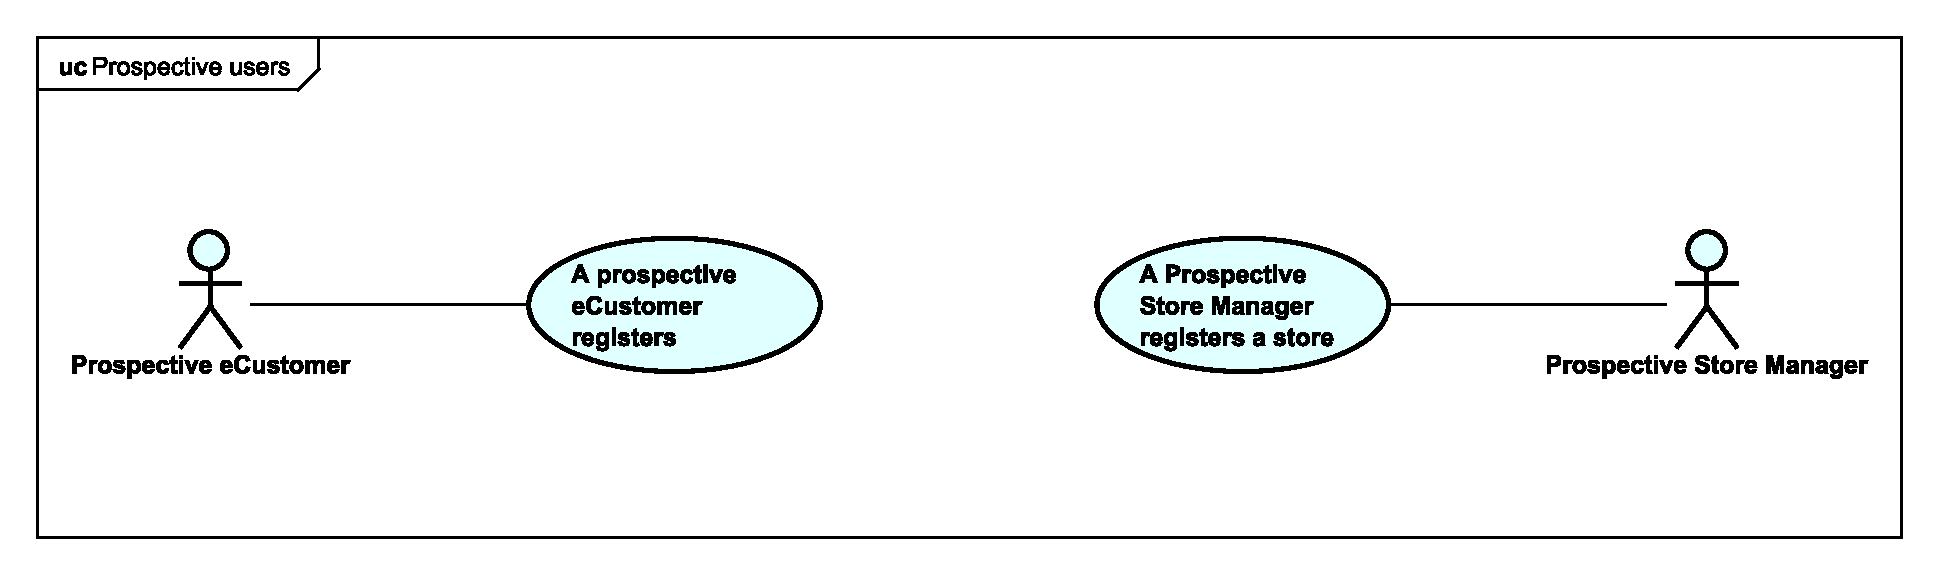
\includegraphics[width=\linewidth] {/use_cases/Prospective_users}
		\caption{Prospective users use cases}
		\label{prospective} }
	{	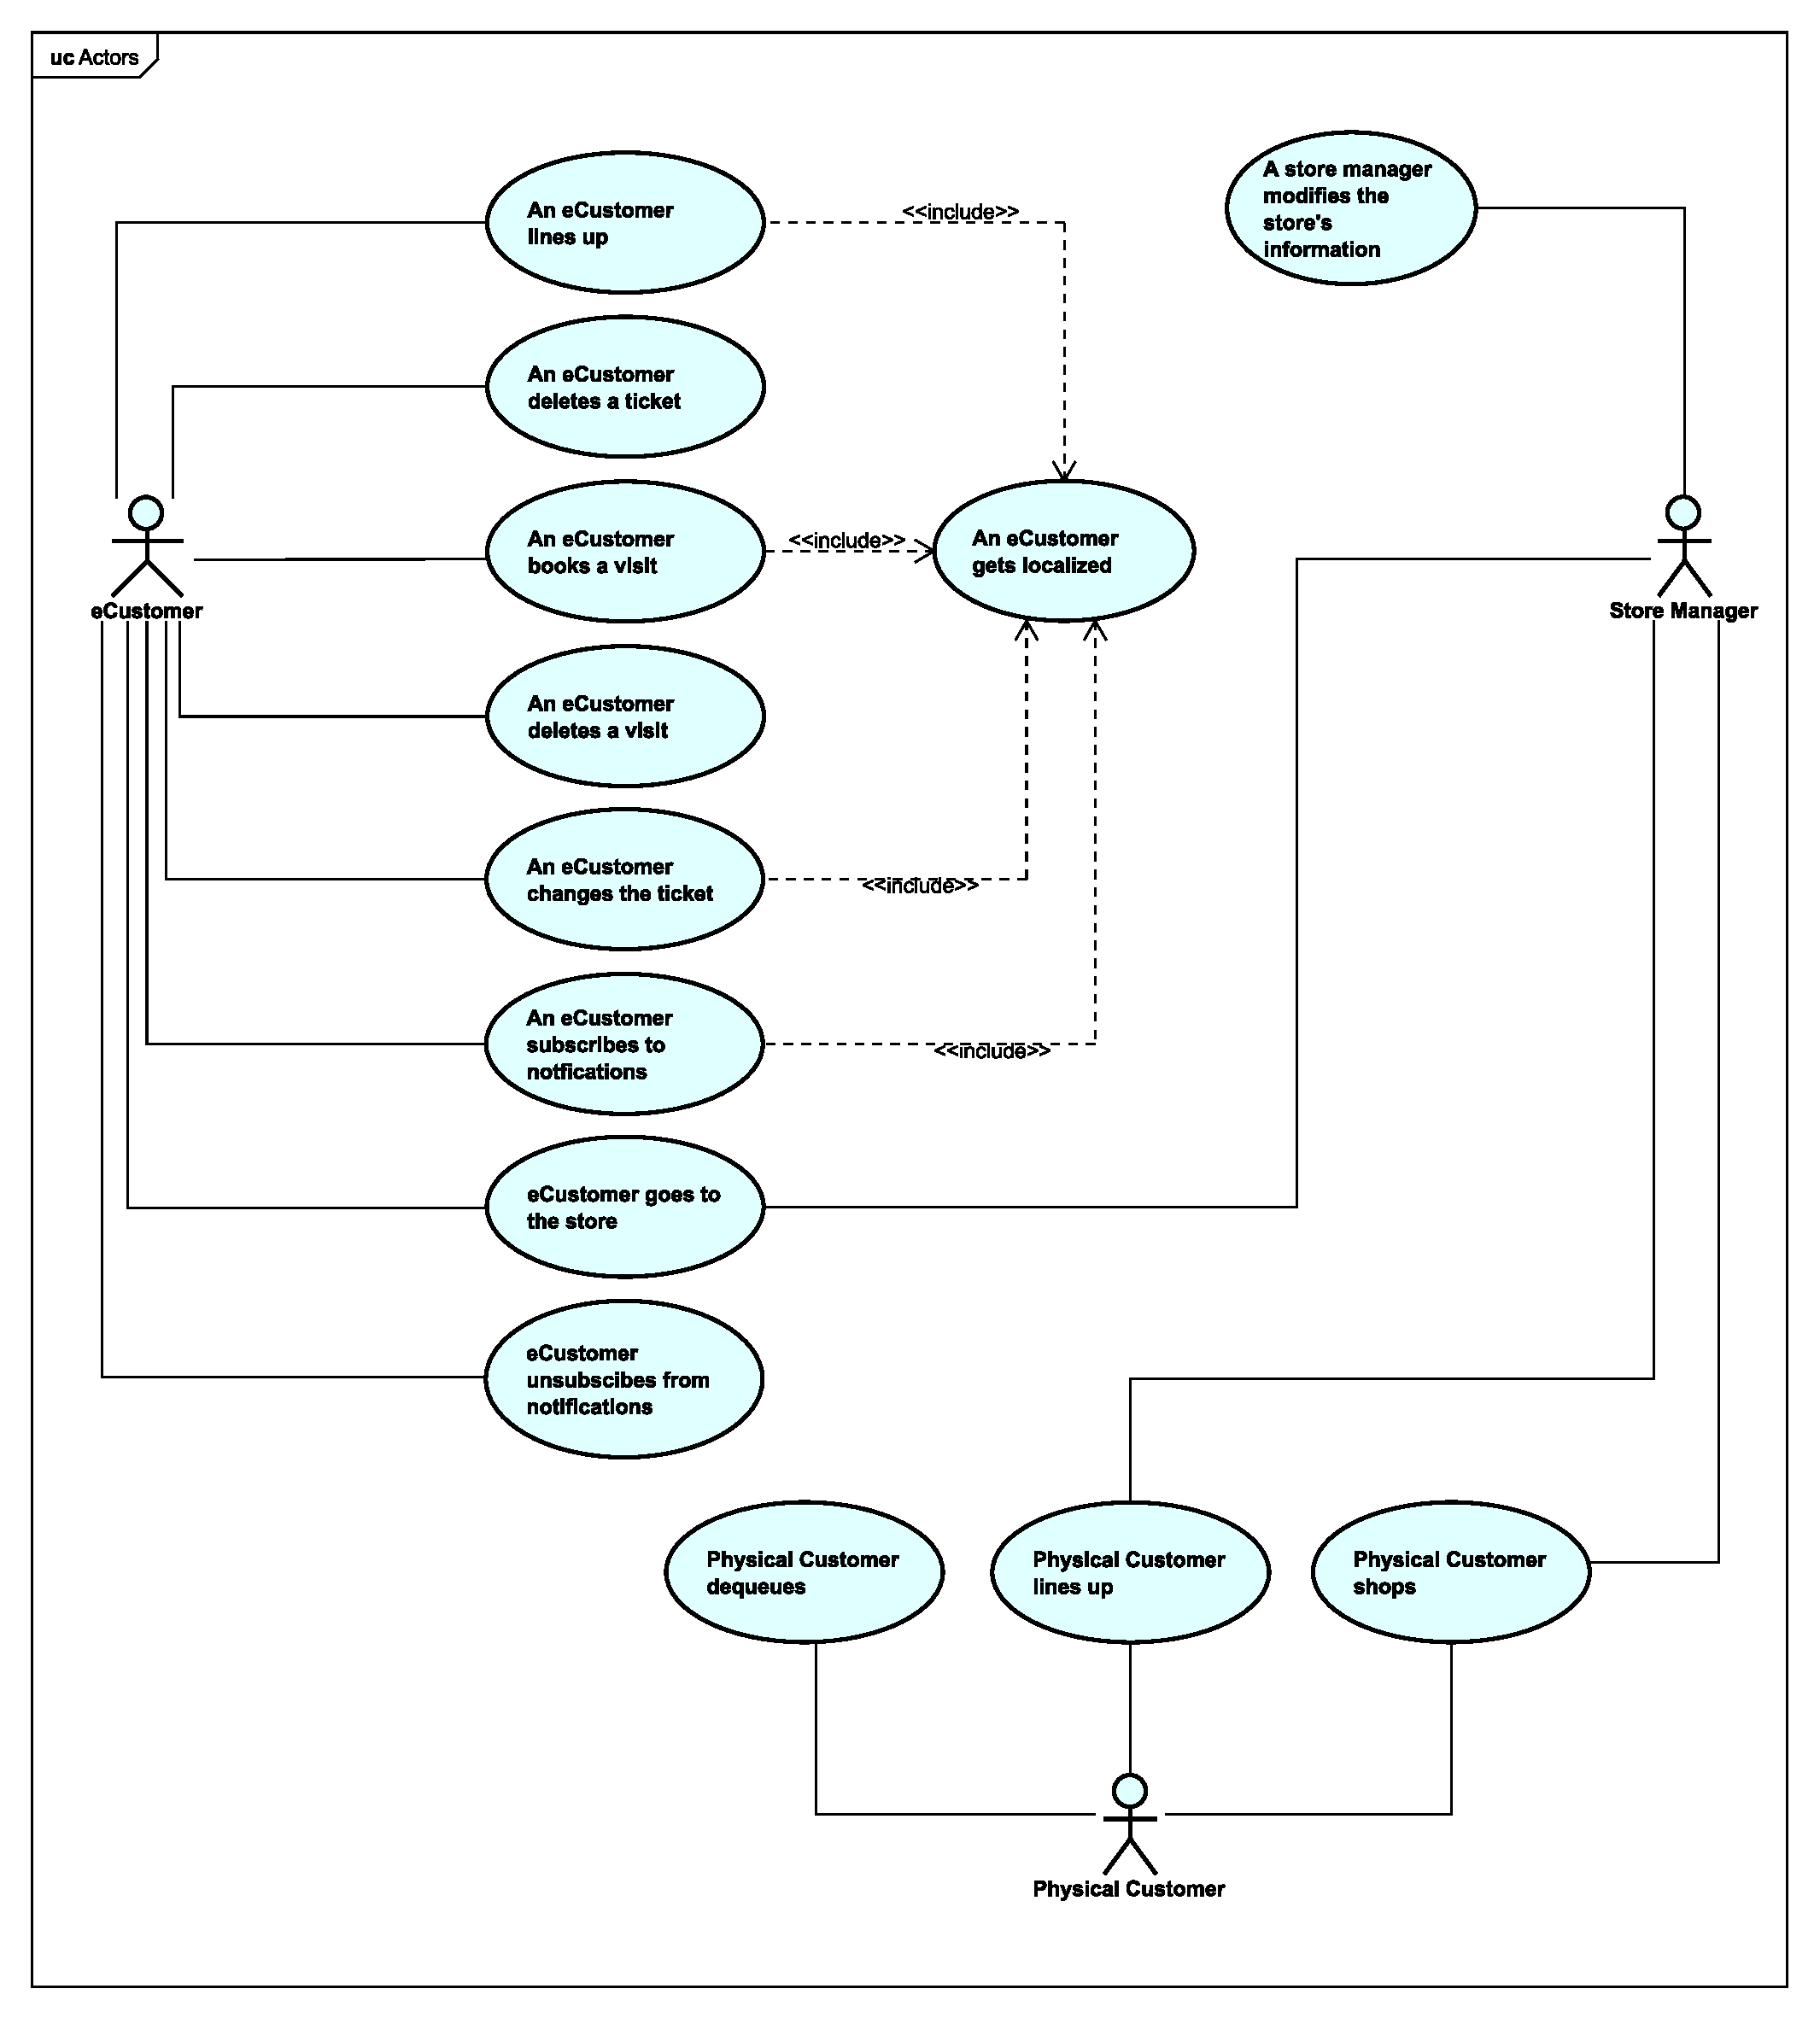
\includegraphics[width=\linewidth] {/use_cases/Actors}
		\caption{Actors use cases}
		\label{uc_actors} }
\end{figure}
\clearpage

% Sequence diagram file, to be included in requirements.tex

\subsection{Sequence diagrams}
Some sequence diagrams:

\begin{figure}[h]
	\centering	
	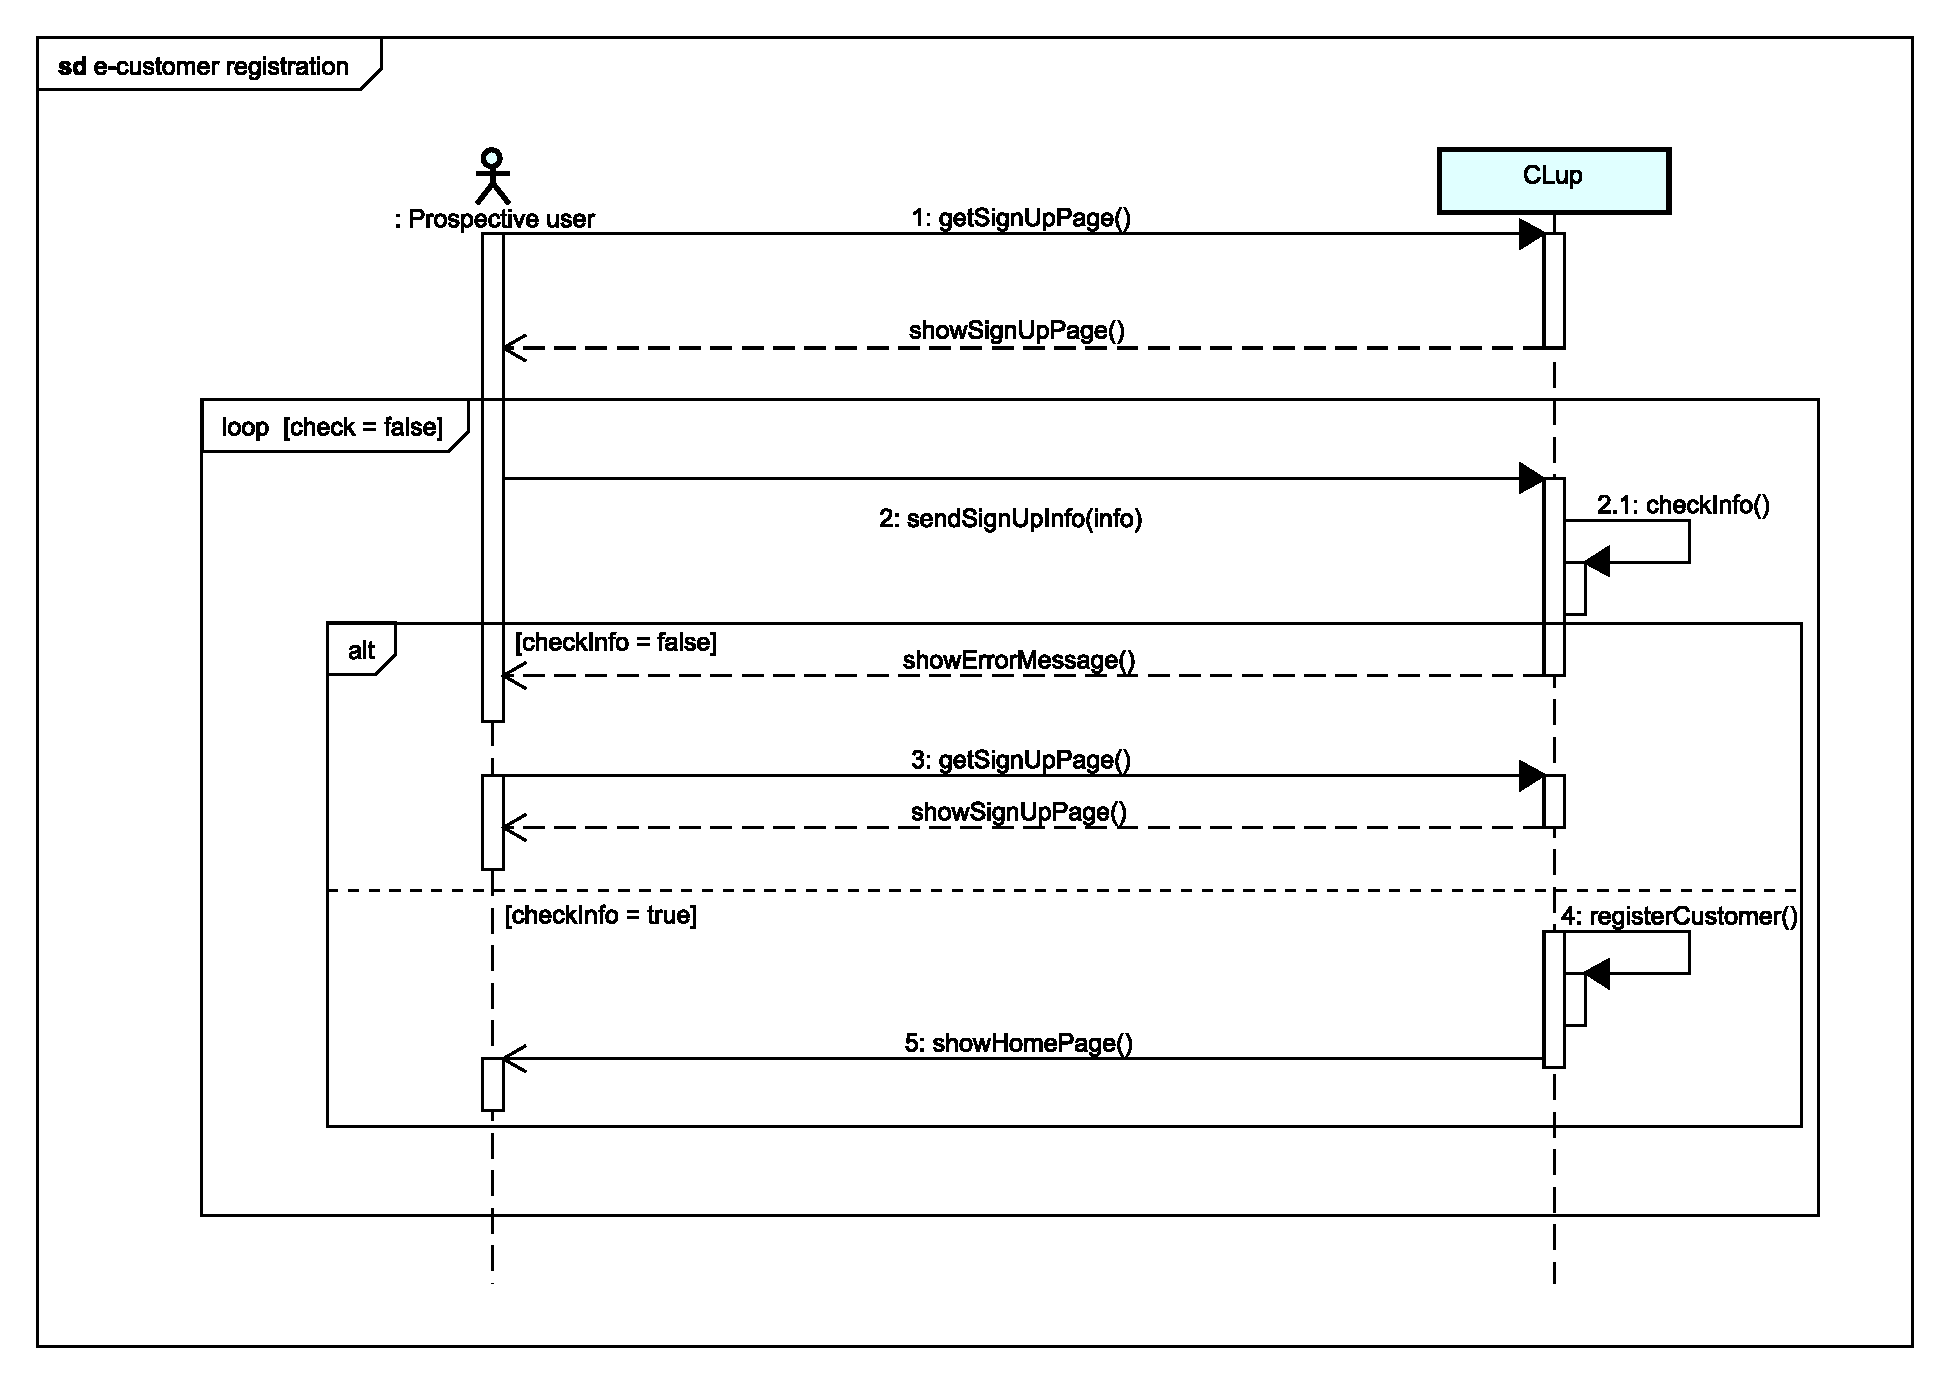
\includegraphics[width=\linewidth] {sequence_diagrams/e-customer_registration}
	\caption{e-Customer registration}
	\label{ec_reg} 
\end{figure}
\clearpage
\begin{figure}[h]
	\centering	
	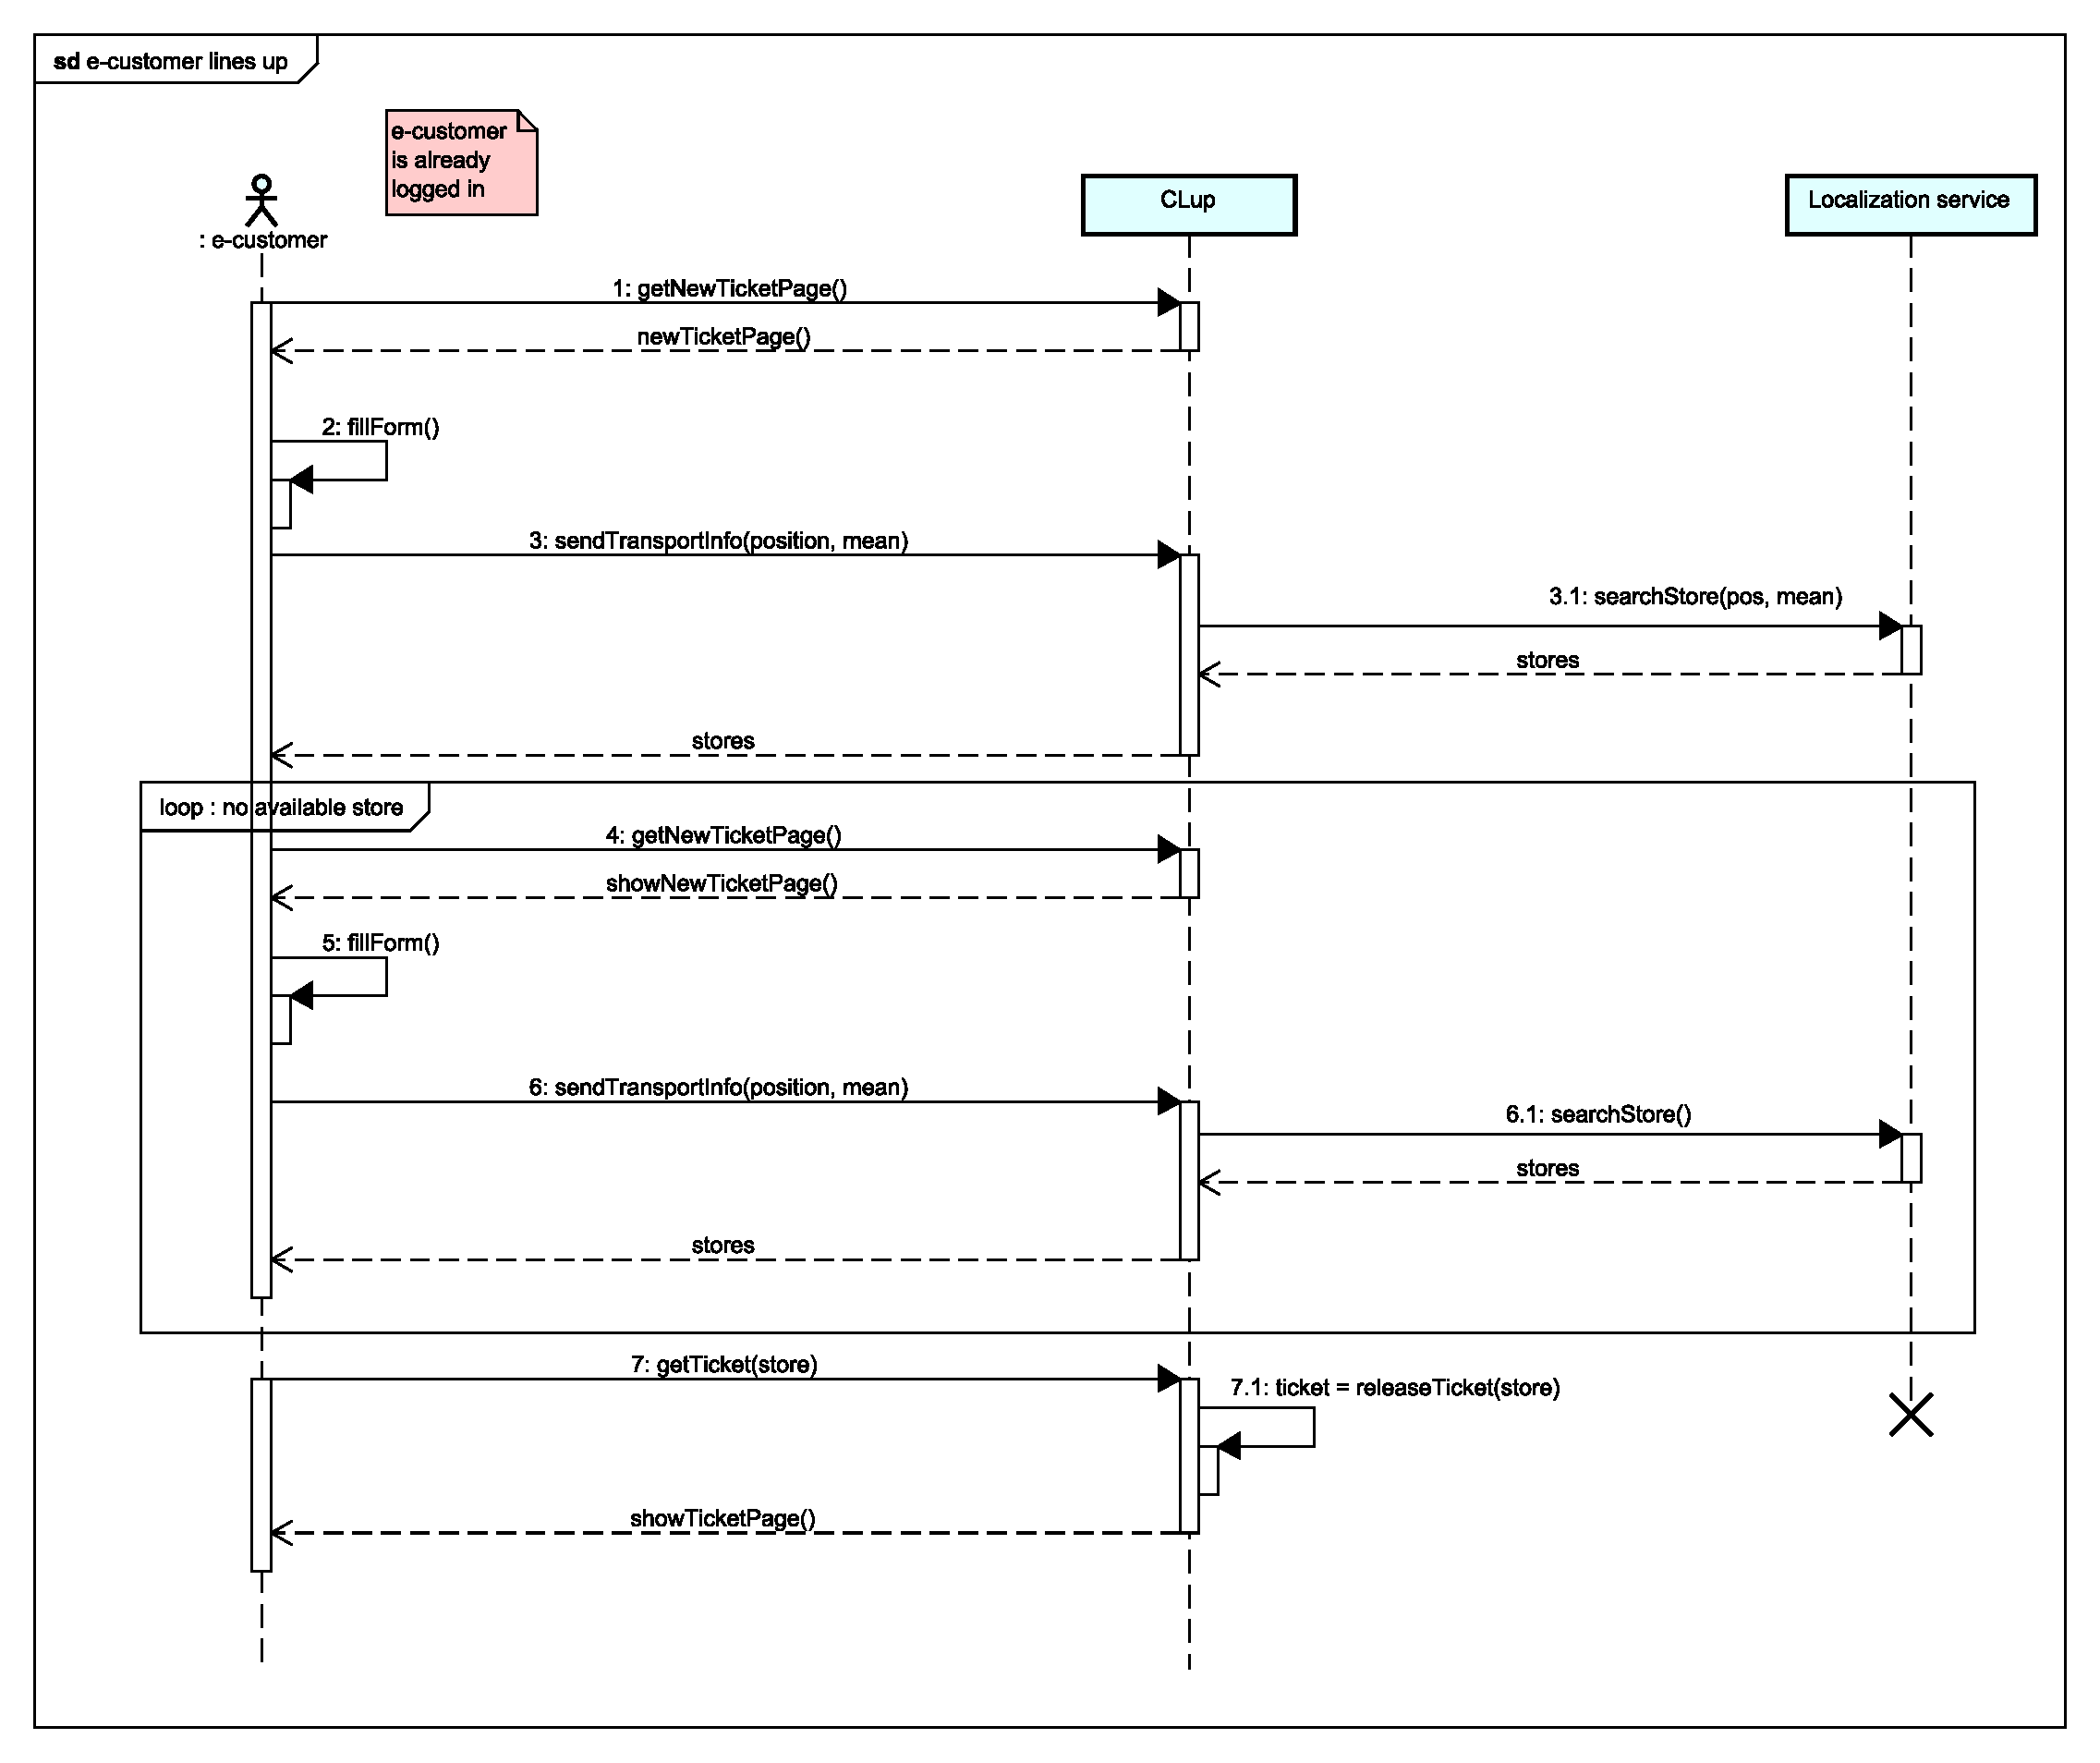
\includegraphics[width=\linewidth] {sequence_diagrams/e-customer_lines_up}
	\caption{e-Customer lines up}
	\label{ec_lup} 
\end{figure}
\clearpage
\begin{figure}[h]
	\centering	
	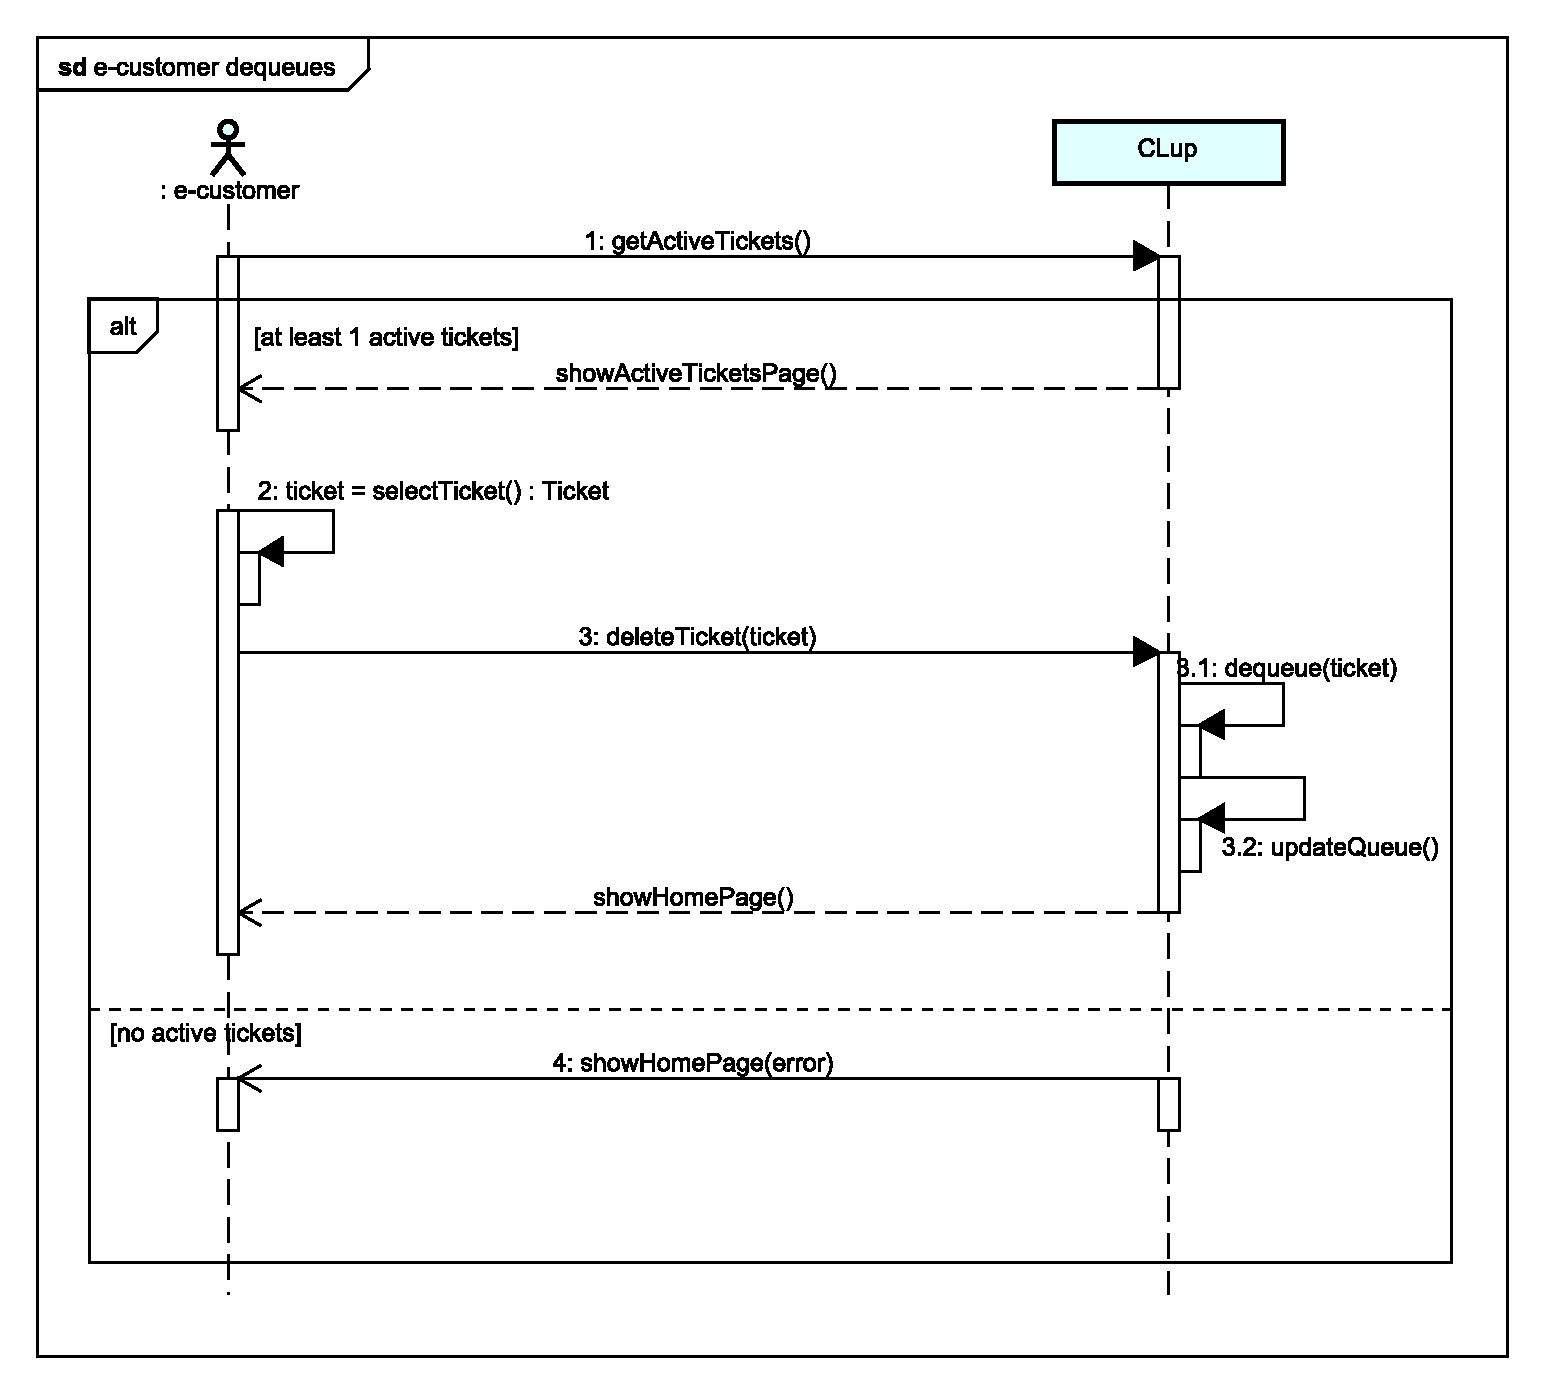
\includegraphics[width=\linewidth] {sequence_diagrams/e-customer_dequeues}
	\caption{e-Customer dequeues}
	\label{ec_deq} 
\end{figure}
\clearpage
\begin{figure}[h]
	\centering	
	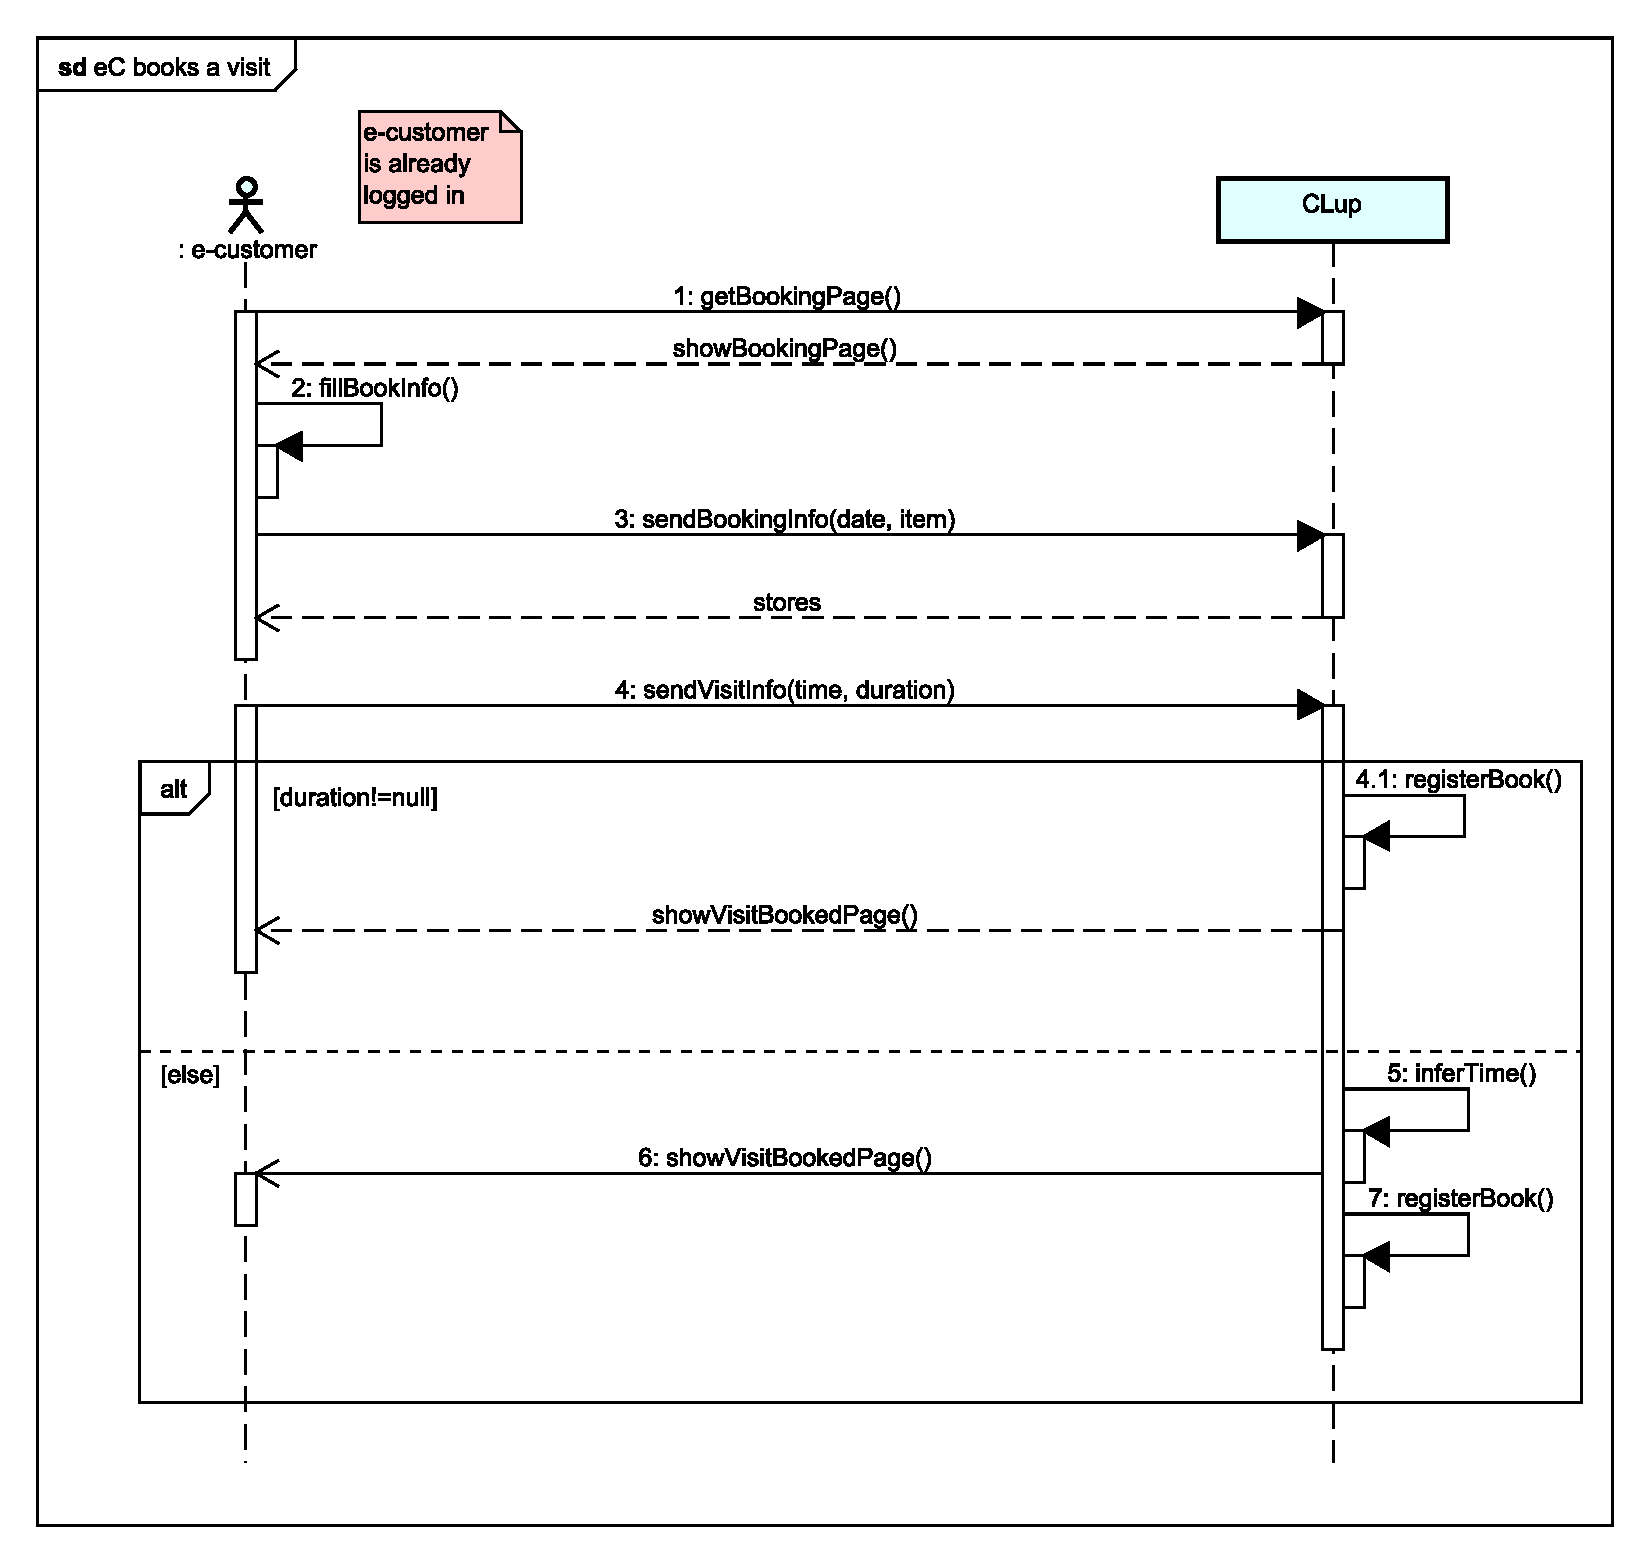
\includegraphics[width=\linewidth] {sequence_diagrams/eC_books_a_visit}
	\caption{e-Customer books a visit}
	\label{ec_book} 
\end{figure}
\clearpage
\begin{figure}[h]
	\centering	
	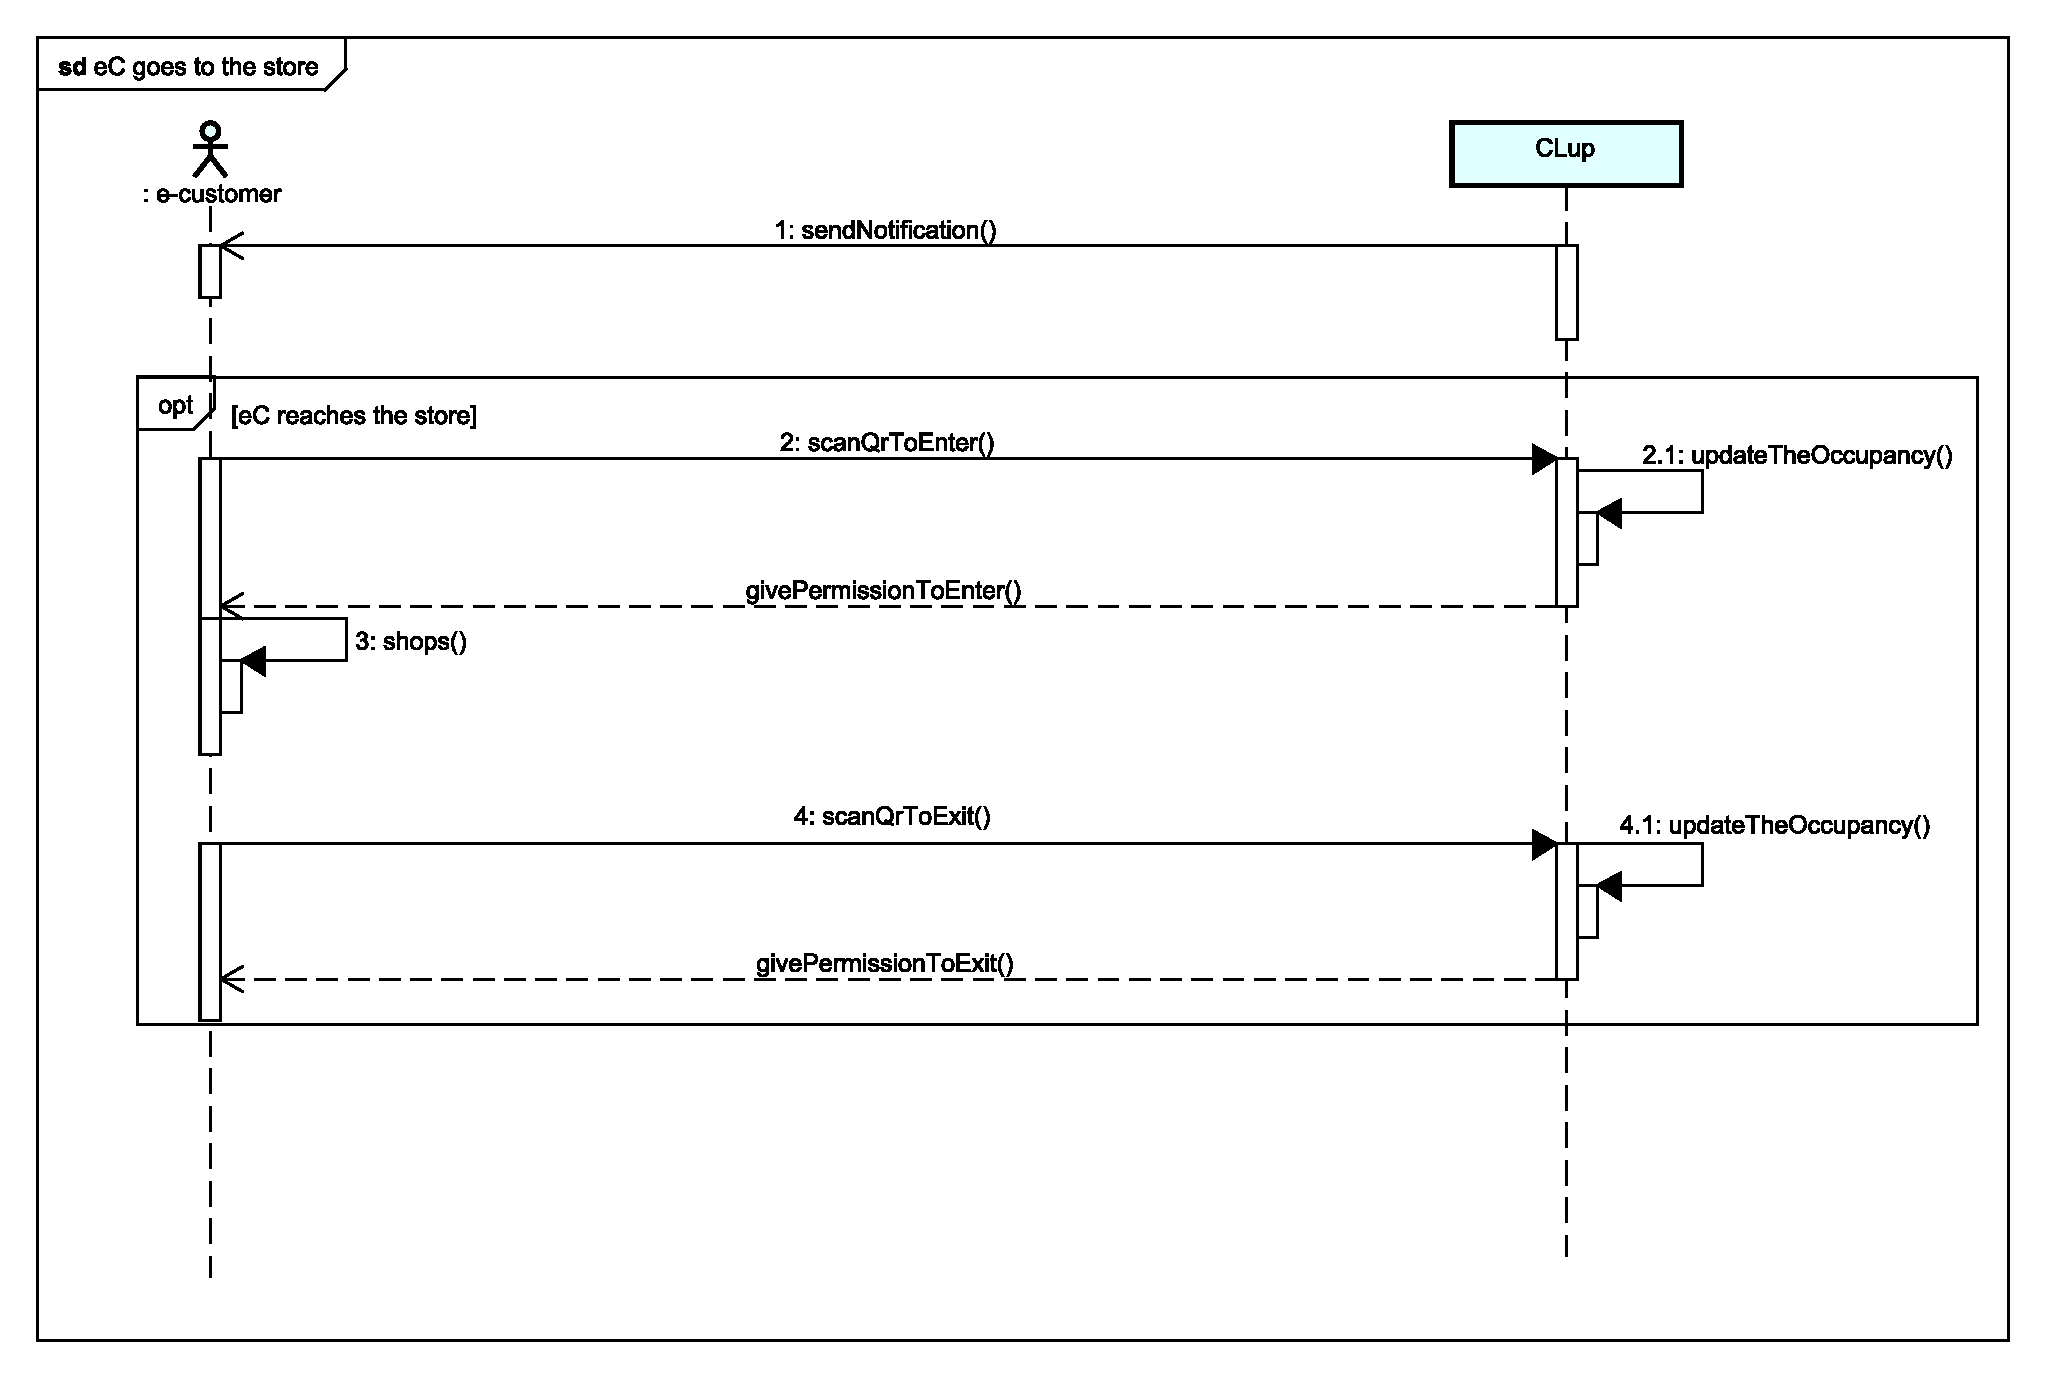
\includegraphics[width=\linewidth] {sequence_diagrams/eC_goes_to_the_store}
	\caption{e-Customer goes to the store}
	\label{ec_store} 
\end{figure}


% Goal, requirements and domains mapping. To be included in requirements.tex

\subsection{Goal Mapping}
In this section, goals are mapped to requirements and domain assumptions.

\subsubsection{[G0] Allow prospective e-Customers to register to the application}
\begin{itemize}
	\setlength\itemsep{-1mm}
	\item [\textbf{[R0]}] Must allow users to provide credentials
	\item [\textbf{[R1]}] Username must be unique 
	\\
	\item [\textbf{[D0]}] Prospective users will complete the registration process
	\item [\textbf{[D3]}] Information provided by users upon registration is correct
	\item [\textbf{[D11]}] The internet connection is always working
\end{itemize}

\subsubsection{[G1] Allow Prospective Store Managers to register to the application by adding their store}
\begin{itemize}
	\setlength\itemsep{-1mm}
	\item [\textbf{[R0]}] Must allow users to provide credentials
	\item [\textbf{[R1]}] Username must be unique 
	\item [\textbf{[R2]}] Store id must be unique
	\item [\textbf{[R3]}] Must allow store managers to add or modify their store’s information
	\\
	\item [\textbf{[D0]}] Prospective users will complete the registration process
	\item [\textbf{[D3]}] Information provided by users upon registration is correct
	\item [\textbf{[D7]}] Information about stores inserted by SMs is correct
	\item [\textbf{[D11]}] The internet connection is always working
\end{itemize}

\subsubsection{[G2] Allow e-customers to line up from home}
\begin{itemize}
	\setlength\itemsep{-1mm}
	\item [\textbf{[R4]}] Users must be able to login
	\item [\textbf{[R5]}] Must be able to provide the list of available stores in the user’s proximity
	\item [\textbf{[R6]}] Must know the e-Customer’s position
	\begin{itemize}[itemsep=-1mm, topsep=-1mm]
		\item [\textbf{[R6.1]}] Must localize the e-Customer or let them provide manually a position
	\end{itemize}
	\item [\textbf{[R7]}] Must assign a unique and sequential reservation id
	\item [\textbf{[R8]}] Must generate a QR code to be scanned at entrance and exit
	\item [\textbf{[R9]}] Must let e-Customers choose their mean of transport
	\item [\textbf{[R10]}] Must allow the entrance when it is the customer’s turn
	\item [\textbf{[R11]}] Must allow a delay of at most M minutes on a customer’s turn
	\item [\textbf{[R12]}] Must show e-Customers the number of enqueued customers in front of them
	\item [\textbf{[R13]}] Must show users historical data on given weekdays
	\item [\textbf{[R14]}] At least P% places must be reserved for tickets
	\item [\textbf{[R15]}] Must notify e-Customers within a suitable time from entrance
	\begin{itemize}[itemsep=-1mm, topsep=-1mm]
		\item [\textbf{[R15.1]}] Notification time must be based on current store occupation 
		\item [\textbf{[R15.2]}] Notification time must be based on estimated travel time
	\end{itemize}
	\item [\textbf{[R16]}] Must let e-Customers advance if a preceding customer dequeued
	\\
	\item [\textbf{[D1]}] Only people enqueued access the stores (both app and physical)
	\item [\textbf{[D2]}] Information provided by e-customers corresponds to their will
	\item [\textbf{[D4]}] Customers enter only if allowed by the application
	\item [\textbf{[D5]}] Customers respect the choices made during the input phase
	\item [\textbf{[D6]}] Calculated travel time is correct
	\item [\textbf{[D7]}] Information about stores inserted by SMs is correct
	\item [\textbf{[D8]}] Customers entering a store exit after some time
	\item [\textbf{[D9]}] If a client exits at a given time, he must have entered in the same opening period
	\item [\textbf{[D10]}] Ticket printers and QR readers work properly
	\item [\textbf{[D11]}] The internet connection is always working
	\item [\textbf{[D12]}] Users accept to receive notifications from the application
	\item [\textbf{[D13]}] Stores show the current customer number
	\item [\textbf{[D14]}] The external web mapping system is always available and there is signal
\end{itemize}

\subsubsection{[G2.1] Allow e-Customers to dequeue}
\begin{itemize}
	\setlength\itemsep{-1mm}
	\item [\textbf{[R4]}] Users must be able to login
	\\
	\item [\textbf{[D11]}] The internet connection is always working
\end{itemize}

\subsubsection{[G3] Allow Store Managers to monitor entrances}
\begin{itemize}
	\setlength\itemsep{-1mm}
	\item [\textbf{[R3]}] Must allow store managers to add or modify their store’s information
	\item [\textbf{[R4]}] Users must be able to login
	\item [\textbf{[R17]}] Must keep track of people inside the stores
	\begin{itemize}[itemsep=-1mm, topsep=-1mm]
		\item [\textbf{[R17.1]}] Must allow scanning QR codes on entrance and exit
	\end{itemize}
	\item [\textbf{[R18]}] Must not allow the entrance of more customers than prescribed
	\\
	\item [\textbf{[D1]}] Only people enqueued access the stores (both app and physical)
	\item [\textbf{[D4]}] Customers enter only if allowed by the application
	\item [\textbf{[D5]}] Customers respect the choices made during the input phase
	\item [\textbf{[D7]}] Information about stores inserted by SMs is correct
	\item [\textbf{[D8]}] Customers entering a store exit after some time
	\item [\textbf{[D9]}] If a client exits at a given time, he must have entered in the same opening period
	\item [\textbf{[D10]}] Ticket printers and QR readers work properly
	\item [\textbf{[D11]}] The internet connection is always working
	\item [\textbf{[D13]}] Stores show the current customer number
\end{itemize}

\subsubsection{[G4] Allow customers to physically line up}
\begin{itemize}
	\setlength\itemsep{-1mm}
	\item [\textbf{[R7]}] Must assign a unique and sequential reservation id
	\item [\textbf{[R8]}] Must generate a QR code to be scanned at entrance and exit
	\item [\textbf{[R10]}] Must allow the entrance when it is the customer’s turn
	\item [\textbf{[R11]}] Must allow a delay of at most M minutes on a customer’s turn
	\item [\textbf{[R20]}] Physical tickets must be placed on the same queue as virtual ones
	\item [\textbf{[R21]}] Physical tickets must be printed
	\\
	\item [\textbf{[D1]}] Only people enqueued access the stores (both app and physical)
	\item [\textbf{[D4]}] Customers enter only if allowed by the application
	\item [\textbf{[D8]}] Customers entering a store exit after some time
	\item [\textbf{[D9]}] If a client exits at a given time, he must have entered in the same opening period
	\item [\textbf{[D10]}] Ticket printers and QR readers work properly
	\item [\textbf{[D11]}] The internet connection is always working
	\item [\textbf{[D13]}] Stores show the current customer number
\end{itemize}

\subsubsection{[G4.1] Allow Physical Customers to dequeue}
\begin{itemize}
	\setlength\itemsep{-1mm}
	\item [\textbf{[R11]}] Must allow a delay of at most M minutes on a customer’s turn
	\item [\textbf{[R22]}] Must allow Physical Customers to scan their code in order to dequeue
	\\
	\item [\textbf{[D10]}] Ticket printers and QR readers work properly
	\item [\textbf{[D11]}] The internet connection is always working
	\item [\textbf{[D13]}] Stores show the current customer number
\end{itemize}

\subsubsection{[G5] Allow e-Customers to book a visit}
\begin{itemize}
	\setlength\itemsep{-1mm}
	\item [\textbf{[R4]}] Users must be able to login
	\item [\textbf{[R5]}] Must be able to provide the list of available stores in the user’s proximity
	\item [\textbf{[R6]}] Must know the e-Customer’s position
	\begin{itemize}[itemsep=-1mm, topsep=-1mm]
		\item [\textbf{[R6.1]}] Must localize the e-Customer or let them provide manually a position
	\end{itemize}
	\item [\textbf{[R7]}] Must assign a unique and sequential reservation id
	\item [\textbf{[R8]}] Must generate a QR code to be scanned at entrance and exit
	\item [\textbf{[R9]}] Must let e-Customers choose their mean of transport
	\item [\textbf{[R10]}] Must allow the entrance when it is the customer’s turn
	\item [\textbf{[R11]}] Must allow a delay of at most M minutes on a customer’s turn
	\item [\textbf{[R13]}] Must show users historical data on given weekdays
	\item [\textbf{[R14]}] At least P\% places must be reserved for tickets
	\item [\textbf{[R15]}] Must notify e-Customers within a suitable time from entrance
	\begin{itemize}[itemsep=-1mm, topsep=-1mm]
		\item [\textbf{[R15.2]}] Notification time must be based on estimated travel time
	\end{itemize}
	\item [\textbf{[R23]}] e-Customers who book a visit must be allowed to enter at their chosen time
	\item [\textbf{[R24]}] Must let e-Customers insert the expected duration of the visit
	\begin{itemize}[itemsep=-1mm, topsep=-1mm]
		\item [\textbf{[R24.1]}] Must be able to infer and suggest the duration for long term customers
	\end{itemize}
	\item [\textbf{[R25]}] Must let e-Customers insert a list of items/categories they intend to buy
	\\
	\item [\textbf{[D1]}] Only people enqueued access the stores (both app and physical)
	\item [\textbf{[D2]}] Information provided by e-customers corresponds to their will
	\item [\textbf{[D4]}] Customers enter only if allowed by the application
	\item [\textbf{[D5]}] Customers respect the choices made during the input phase
	\item [\textbf{[D6]}] Calculated travel time is correct
	\item [\textbf{[D7]}] Information about stores inserted by SMs is correct
	\item [\textbf{[D8]}] Customers entering a store exit after some time
	\item [\textbf{[D10]}] Ticket printers and QR readers work properly
	\item [\textbf{[D11]}] The internet connection is always working
	\item [\textbf{[D12]}] Users accept to receive notifications from the application
	\item [\textbf{[D14]}] The external web mapping system is always available and there is signal
\end{itemize}

\subsubsection{[G5.1] Allow e-Customers to delete a visit}
\begin{itemize}
	\setlength\itemsep{-1mm}
	\item [\textbf{[R4]}] Users must be able to login
	\\
	\item [\textbf{[D11]}] The internet connection is always working
\end{itemize}

\subsubsection{[G6] Can suggest alternative slots to balance the number of customers}
\begin{itemize}
	\setlength\itemsep{-1mm}
	\item [\textbf{[R4]}] Users must be able to login
	\item [\textbf{[R6]}] Must know the e-Customer’s position
	\begin{itemize}[itemsep=-1mm, topsep=-1mm]
		\item [\textbf{[R6.1]}] Must localize the e-Customer or let them provide manually a position
	\end{itemize}
	\item [\textbf{[R17]}] Must keep track of people inside the stores
	\item [\textbf{[R26]}] Alternatives must be based on information provided by the e-Customer and store occupation (both real time and historical)
	\\
	\item [\textbf{[D4]}] Customers enter only if allowed by the application
	\item [\textbf{[D5]}] Customers respect the choices made during the input phase
	\item [\textbf{[D6]}] Calculated travel time is correct
	\item [\textbf{[D7]}] Information about stores inserted by SMs is correct
	\item [\textbf{[D8]}] Customers entering a store exit after some time
	\item [\textbf{[D9]}] If a client exits at a given time, he must have entered in the same opening period
	\item [\textbf{[D11]}] The internet connection is always working
	\item [\textbf{[D14]}] The external web mapping system is always available and there is signal
\end{itemize}

\subsubsection{[G7] Allow e-Customers to manage slot notifications}
\begin{itemize}
	\setlength\itemsep{-1mm}
	\item [\textbf{[R4]}] Users must be able to login
	\item [\textbf{[R6]}] Must know the e-Customer’s position
	\begin{itemize}[itemsep=-1mm, topsep=-1mm]
		\item [\textbf{[R6.1]}] Must localize the e-Customer or let them provide manually a position
	\end{itemize}
	\item [\textbf{[R17]}] Must keep track of people inside the stores
	\item [\textbf{[R27]}] e-Customers must be able to subscribe to the notification service
	\item [\textbf{[R28]}] Must let e-Customers unsubscribe from the notification service
	\item [\textbf{[R29]}] The system must notify the e-Customers based on their choices
	\\
	\item [\textbf{[D2]}] Information provided by e-customers corresponds to their will
	\item [\textbf{[D7]}] Information about stores inserted by SMs is correct
	\item [\textbf{[D8]}] Customers entering a store exit after some time
	\item [\textbf{[D9]}] If a client exits at a given time, he must have entered in the same opening period
	\item [\textbf{[D11]}] The internet connection is always working
	\item [\textbf{[D12]}] Users accept to receive notifications from the application
	\item [\textbf{[D14]}] The external web mapping system is always available and there is signal
\end{itemize}

% Non-functional requirements page, to be included in requirements.tex

\subsection{Non-functional requirements}
An important non-functional requirement is the ease of use, given the wide variety of people potentially using the system. Requirements related to the system are as follows.

\subsubsection{Performance}
CLup, both for the app and the web application, should provide fast responses to user actions, possibly under 3 seconds\textsuperscript{\cite{speed}}. This result should account for about 150000 daily requests, based on competitor's data\textsuperscript{\cite{ufirst}}.

\subsubsection{Availability and reliability}
As a service used for primary needs connected to stores potentially open all day and every period of the year, CLup should be very robust and reliable, offering an availability of at least 0.999 (that corresponds to less than a day of downtime every year).

\subsubsection{Security}
All user information will need to be securely stored by the application. The communication between clients and server should be protected alongside QR codes, in order to ensure fairness in queue management too.

\subsubsection{Maintainability}
As in all software applications, maintainability should be a core property of CLup, enabling changes both related to modifications in functionalities and bug fixing.

\subsubsection{Portability}
The client system should be developed to be compatible with most of the mobile Operating Systems (for the mobile application) and browsers (for the web app). The latter option should prioritize mobile environments (i.e. smartphones, tablets) without precluding access to desktop-based systems, even if they are not the primary target of the application.

% Design constraints page, to be included in requirements.tex

\subsection{Design constraints}

\subsubsection{Hardware and software limitations}
The hardware and software requirements are stated here, divided by usage:
\begin{itemize}[itemsep=-1mm, topsep=-1mm]
	\item For the mobile application: 
	\begin{itemize}[itemsep=-1mm, topsep=-1mm]
		\item Operating system: Android 6.0+ or iOS 9+
		\item The device must be internet enabled
	\end{itemize}
	
	\item For the web application, a device with either:
	\begin{itemize}[itemsep=-1mm, topsep=-1mm]
		\item Mozilla Firefox 19.0+
		\item Google Chrome 25.0+
		\item Microsoft Edge 
		\item Safari 5.1+
		\item Opera 12.1+
	\end{itemize}
\end{itemize}	
A mobile device used by a Store Manager will also need a camera.

\subsubsection{Privacy policies}
The system will need to access some device data in order to function properly; the following table summarizes the permission requests:

\begin{center}
	\rowcolors{4}{white}{tablerow}
	\begin{tabular}{c | c | c | c | c }
		\multirow{2}{*}{Permission} & \multicolumn{2}{c|}{e-Customer} & \multicolumn{2}{c}{Store Manager} \\ \cline{2-5}
		                            & Mobile & Web                    & Mobile & Web                      \\ \hline
		          Storage           & Mandatory      &                       &       &  \\
		          Camera &  &  & Mandatory & Mandatory \\
		          Localization & Optional & Optional &  & 
	\end{tabular}
\end{center}

Moreover, in order to comply with privacy regulations\textsuperscript{\cite{gdpr}}, CLup:
\begin{itemize}[itemsep=-1mm, topsep=-1mm]
	\item Will ask for the user's consent for their data processing
	\item Will not use any of the user data for purposes different from the offered service
	\item Will not request personal data that is not necessary to offer the service
	\item Will not keep any personal data once it is not needed anymore
	\item Will ensure privacy and security by design
\end{itemize}


